\documentclass[aspectratio=169, 12pt]{beamer}
\usepackage[utf8]{inputenc}
\usepackage[T1]{fontenc}
\usepackage[brazil]{babel}
\usepackage{lmodern}
\usepackage{amsmath, amssymb, amsfonts}
\usepackage{graphicx}
\usepackage{booktabs}        
\usepackage{multirow}
\usepackage{xcolor}
\usepackage{tikz}
\usetikzlibrary{arrows.meta, positioning, shapes.geometric}
\usepackage{pgfplots}
\pgfplotsset{compat=1.18}
\usepackage{hyperref}
\usepackage{natbib}          
\usepackage{caption}
\usepackage{subcaption}
\usepackage{enumitem}
\usepackage{microtype}
\definecolor{EcoNavy}{HTML}{1A2A4A}     
\definecolor{EcoGold}{HTML}{C9A84C}      
\definecolor{EcoMid}{HTML}{2E4272}       
\definecolor{EcoLight}{HTML}{EAF0FB}     
\definecolor{EcoGray}{HTML}{6B7A99}      
\definecolor{EcoWhite}{HTML}{F5F7FA}    
\usetheme{Madrid}
\usecolortheme{default}
\setbeamercolor{palette primary}{bg=EcoNavy, fg=white}
\setbeamercolor{palette secondary}{bg=EcoMid, fg=white}
\setbeamercolor{palette tertiary}{bg=EcoGold, fg=EcoNavy}
\setbeamercolor{palette quaternary}{bg=EcoNavy, fg=white}
\setbeamercolor{structure}{fg=EcoNavy}
\setbeamercolor{frametitle}{bg=EcoNavy, fg=white}
\setbeamercolor{title}{bg=EcoNavy, fg=white}
\setbeamercolor{subtitle}{fg=EcoGold}
\setbeamercolor{block title}{bg=EcoNavy, fg=white}
\setbeamercolor{block body}{bg=EcoLight, fg=EcoNavy}
\setbeamercolor{block title alerted}{bg=EcoGold!80!EcoNavy, fg=EcoNavy}
\setbeamercolor{block body alerted}{bg=EcoGold!15, fg=EcoNavy}
\setbeamercolor{block title example}{bg=EcoMid, fg=white}
\setbeamercolor{block body example}{bg=EcoLight, fg=EcoNavy}
\setbeamercolor{item}{fg=EcoGold}
\setbeamercolor{subitem}{fg=EcoMid}
\setbeamercolor{subsubitem}{fg=EcoGray}
\setbeamercolor{footline}{bg=EcoNavy, fg=EcoWhite}
\setbeamercolor{headline}{bg=EcoNavy}
\setbeamercolor{section in head/foot}{bg=EcoNavy, fg=EcoWhite}
\setbeamercolor{subsection in head/foot}{bg=EcoMid, fg=EcoWhite}
\setbeamercolor{page number in head/foot}{fg=EcoGold}


\usefonttheme{professionalfonts}
\setbeamerfont{title}{size=\Large, series=\bfseries}
\setbeamerfont{subtitle}{size=\normalsize, series=\normalfont}
\setbeamerfont{frametitle}{size=\large, series=\bfseries}
\setbeamerfont{framesubtitle}{size=\small, series=\normalfont}
\setbeamertemplate{navigation symbols}{}
 \setbeamertemplate{itemize item}{\(\blacktriangleright\)}
\setbeamertemplate{itemize subitem}{\color{EcoMid}$\blacktriangleright$}
\setbeamertemplate{itemize subsubitem}{\color{EcoGray}$\circ$}

\setbeamertemplate{footline}{%
  \leavevmode%
  \hbox{%
    \begin{beamercolorbox}[wd=.33\paperwidth, ht=2.25ex, dp=1ex, left, leftskip=1em]{section in head/foot}%
      \usebeamerfont{author in head/foot}\insertshortauthor
    \end{beamercolorbox}%
    \begin{beamercolorbox}[wd=.34\paperwidth, ht=2.25ex, dp=1ex, center]{section in head/foot}%
      \usebeamerfont{title in head/foot}\insertshorttitle
    \end{beamercolorbox}%
    \begin{beamercolorbox}[wd=.33\paperwidth, ht=2.25ex, dp=1ex, right, rightskip=1em]{section in head/foot}%
      \usebeamerfont{date in head/foot}\insertshortdate{}\hspace{2em}
      \textcolor{EcoGold}{\insertframenumber{} / \inserttotalframenumber}
    \end{beamercolorbox}%
  }%
  \vskip0pt%
}
\setbeamertemplate{headline}{}
\defbeamertemplate*{title page}{custom}[1][]{%
  \begin{tikzpicture}[remember picture, overlay]
    % Fundo branco
    \fill[white] (current page.south west) rectangle (current page.north east);
  \end{tikzpicture}%
  \vspace{0.4cm}
  \begin{center}
    
\includegraphics[height=3.4cm]{figuras/logo_ufcg_melhor.png}\par
    \vspace{0.7cm}
    {\usebeamerfont{title}\textcolor{EcoNavy}\inserttitle\par}
    \vspace{0.3cm}
    {\usebeamerfont{subtitle}\textcolor{EcoNavy}\insertsubtitle\par}
    \vspace{0.6cm}
    {\small\textcolor{EcoNavy}\insertauthor\par}
    \vspace{0.15cm}
    {\small\textcolor{EcoGray}\insertinstitute\par}
    \vspace{0.6cm}
    {\footnotesize\textcolor{EcoGray}\insertdate\par}
  \end{center}
}
\title {\textbf{Análise Sobre a Crise de 2008}}
\subtitle{ Economia Internacional II}
\author[Arthur Lira, Nathan Sousa]{%
  \begin{tabular}{@{}ll@{}}
    \makebox[2.3cm][l]{\textbf{Alunos:}} & Arthur Henrique Resende Lira \\
    \makebox[2.3cm][l]{}                 & Nathan Pereira Gomes de Sousa \\
    \makebox[2.3cm][l]{\textbf{Professor(a):}} & Luiza Dantas de Souza Lima Teixeira \\
  \end{tabular}
}
\institute[Universidade]{%
  Unidade Academica de Economia e Finanças\\
  Universidade Federal de Campina Grande
}
\date[\today]{Campina Grande, \today}
\begin{document}
\begin{frame}[plain]
  \titlepage
\end{frame}
\begin{frame}[shrink=10]{Sumário}
  \tableofcontents[hideallsubsections]
\end{frame}
\begin{frame}
  \footnotesize
   \begin{columns}[T]
    \column{0.48\textwidth}
      \begin{block}{Definição}
       Evento economico adverso que afetou boa parte do mundo, principalmente o norte global.
      \end{block}
      \begin{block}{Características}
    \begin{itemize}
    \setlength{\itemsep}{2pt}
    \setlength{\parskip}{0pt}
    \setlength{\parsep}{0pt}
        \item Crise de tipo Financeira.
        \item Inicio no mercado imobiliario.
        \item Diretamente ligada com o setor financeiro.
      \end{itemize}
      \end{block}
    \begin{block}{Causa}
A literatura destaca que a crise foi gestada durante a década de oitenta, quando houve um expressivo aumento da oferta de crédito e a partir da desregulamentação do sistema bancario.


\end{block}
\column{0.30\textwidth}

\begin{alertblock}{Consequências}
\small

\begin{center}
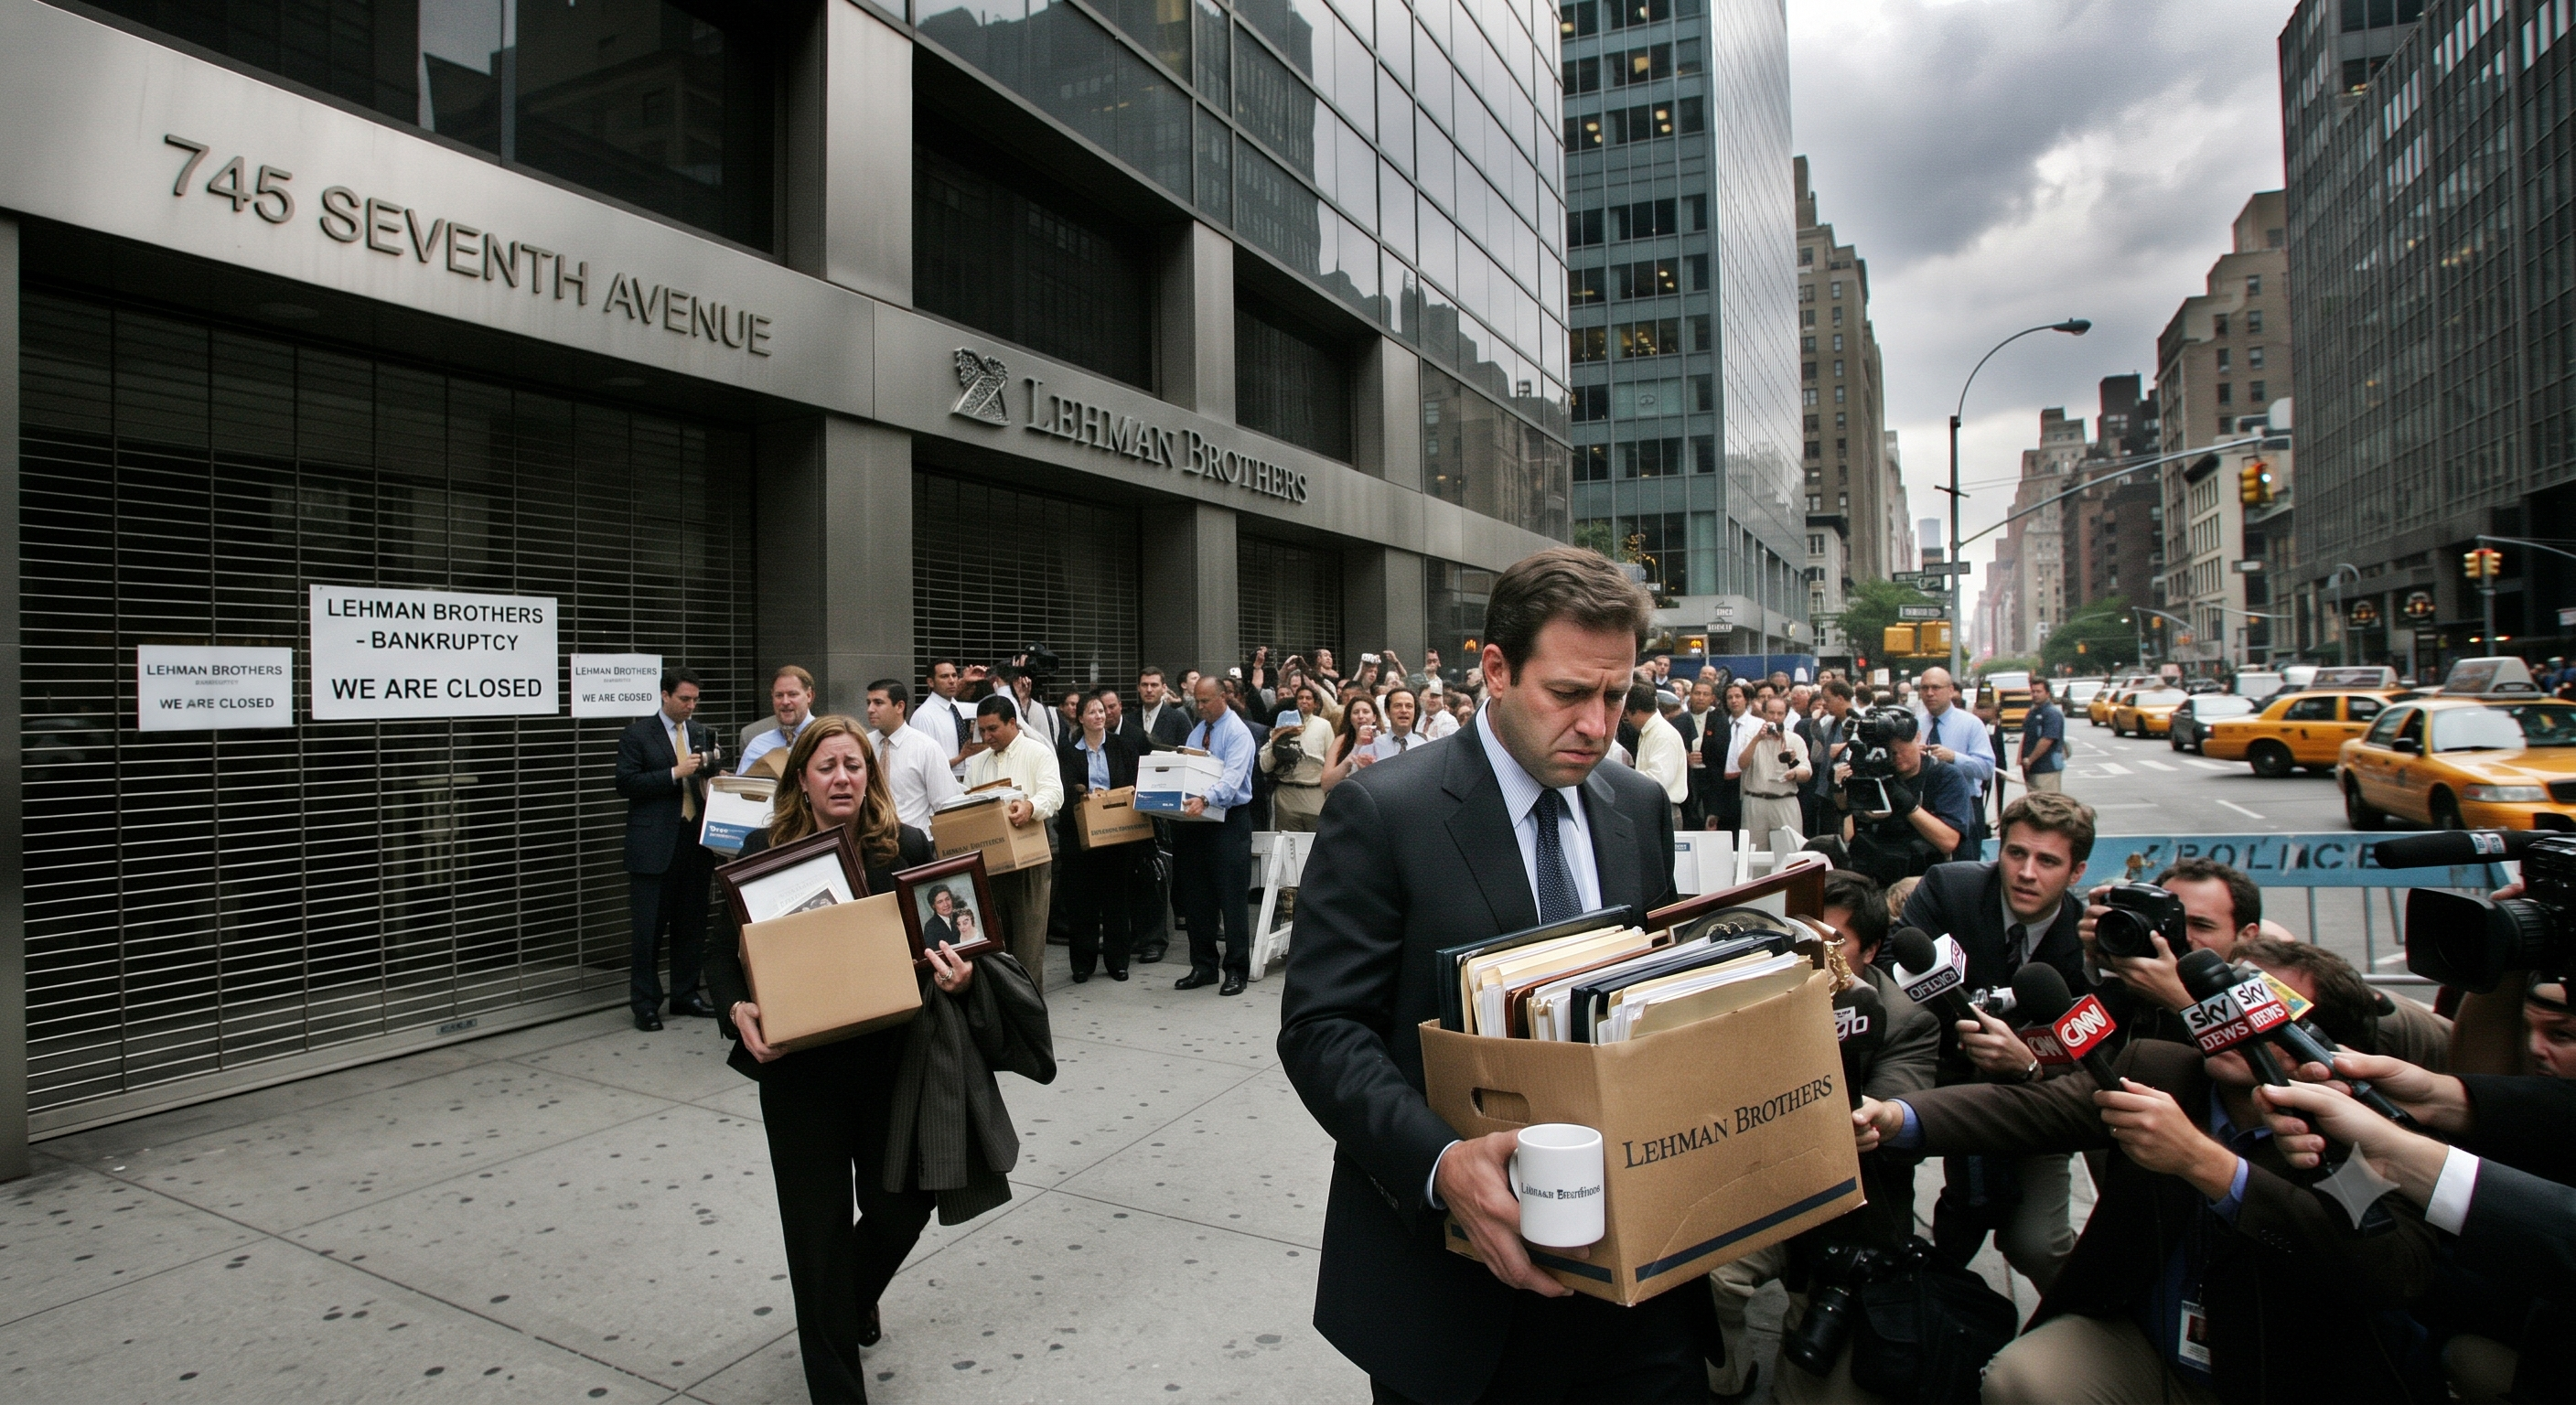
\includegraphics[width=\linewidth]{figuras/LMB.png}
\end{center}

O estouro da bolha levou os Estados Unidos a pior recessão desde 1929, a contração de crédito fez com que os investimentos produtivos despencassem, isso resultou em uma queda drastica do PIB e uma lenta recuperação
\end{alertblock}
\end{columns}
\end{frame}

\begin{frame}
 \begin{columns}

\column{0.55\textwidth}
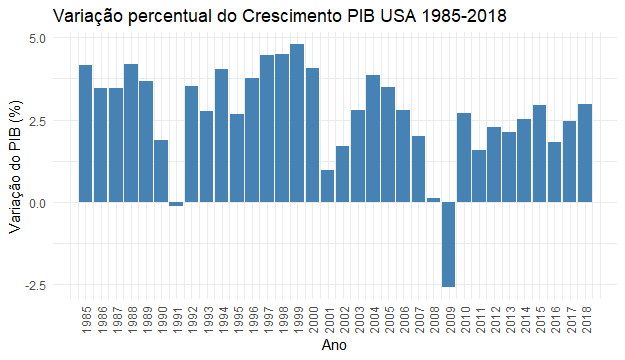
\includegraphics[width=\linewidth]{figuras/Rplot01.png}

\column{0.42\textwidth}
\begin{block}
\scriptsize
O gráfico mostra o crescimento contínuo do PIB americano entre 1985 e 2000 , interrompido pela retração provocada pelo estouro da bolha das empresas \textit{ponto com}. Sob a ótica de Minsky, o período já apresentava sinais de crescente fragilidade financeira. Como resposta à desaceleração, o governo reduziu as taxas de juros, estimulando a expansão do crédito e contribuindo para a formação da bolha imobiliária que culminaria na crise de 2008
\end{block}
\end{columns}
\end {frame}
\begin{frame}{Gestação da Crise}
   \begin{columns}

\column{0.55\textwidth}
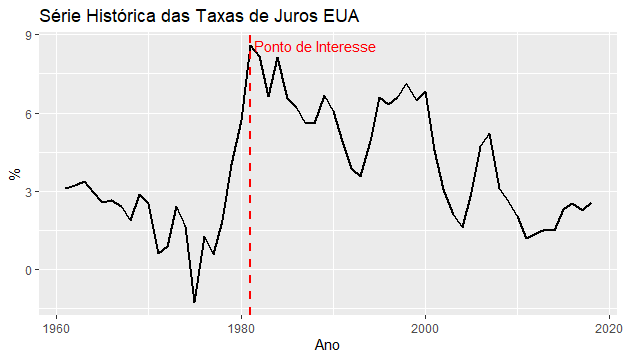
\includegraphics[width=\linewidth]{figuras/jurosUSA.png}

\column{0.42\textwidth}
\begin{block}
\scriptsize
Após 1977, os juros americanos subiram devido à crise do petróleo. Para conter a retração econômica, o governo implementou uma política monetária expansionista: ao reduzir as taxas de juros, buscou injetar liquidez no mercado e incentivar novos investimentos. Ao mesmo passo, a \textbf{Desregulamentação Financeira} daria uma nova cara aos bancos americanos. 

\end{block}

\end{columns}
\end{frame}
\begin{frame}[shrink=13]{Gestação da Crise}
  \framesubtitle{O Papel do Estado e das Instituições Financeiras}
  \begin{columns}[T]

% Coluna da esquerda
\column{0.22\textwidth}

\begin{block}{Ronald Reagan}
\centering


\includegraphics[width=0.65\linewidth]{figuras/RR.jpg}

\vspace{0.4em}

\raggedright
\scriptsize
Presidente dos Estados Unidos entre 1981 e 1989. Seu governo promoveu a desregulamentação financeira, a redução da intervenção estatal e políticas favoráveis ao livre mercado, criando condições para a expansão do sistema financeiro nas décadas seguintes.
\end{block}

\column{0.75\textwidth}


\begin{block}{A Lei Garn-St. Germain Depository Institutions Act of 1982}
A presidência de Reagan redesenhou o sistema financeiro com o afrouxamento da regulação bancária. A lei de 1982, somada à abolição do teto de juros em 1980, permitiu que bancos atuassem em negócios especulativos de alto risco e aumentassem a cobrança de taxas de juros, garantindo maior autonomia operacional ao setor.\end{block}
\begin{alertblock}{Síntese}
O desenvolvimento do sistema bancario dentro dessas perspectivas gerou um terreno amplo para dar vida a crise de 2008. Visto que as operações de risco agora operadas pelos bancos podiam ser vendidas para populações mais vulneraveis (o que futuramente vai aparecer na forma das hipotecas).
\end{alertblock}
 
\end{columns}
\end{frame}
\begin{frame}[shrink=5]{Início}
\framesubtitle{Cenário}

\scriptsize

\begin{columns}[T]

\column{0.40\textwidth}

\begin{block}{Bolha Pontocom}
A chegada aos anos 2000 foi marcada pelo estouro da bolha das empresas \textit{ponto com}. Durante o final da década de 1990, a popularização da internet gerou forte otimismo entre investidores, que direcionaram grandes volumes de capital para startups sem modelos de negócio consolidados, inflando artificialmente o valor dessas empresas.
\end{block}

\column{0.58\textwidth}

\begin{alertblock}{Contenção da Crise}
Para evitar uma recessão mais profunda após o colapso da bolha, o Banco Central dos Estados Unidos adotou uma política monetária expansionista. A taxa básica de juros caiu de aproximadamente 6,5\% em 2001 para 1\% entre 2003 e 2004, permanecendo em níveis historicamente baixos por vários anos. Esse cenário estimulou a expansão do crédito, especialmente no mercado imobiliário, contribuindo para a formação da bolha que culminaria na crise de 2008.
\end{alertblock}
\vspace{0.3em}

\begin{exampleblock}{Resultados}
\scriptsize
A manutenção dos juros em níveis reduzidos incentivou uma forte expansão do crédito imobiliário. Bancos e investidores passaram a concentrar suas operações em hipotecas \textit{subprime}, concedidas a famílias de maior risco por meio de contratos com "taxas teaser". Como esses financiamentos eram rapidamente vendidos e securitizados, a preocupação com a capacidade de pagamento dos mutuários tornou-se secundária, favorecendo a formação da bolha imobiliária.
\end{exampleblock}
\end{columns}

\end{frame}
\begin{frame}{Chegada a 2008}
\framesubtitle{Contextualização}
\begin{columns}[T]

\column{0.49\textwidth}
\centering
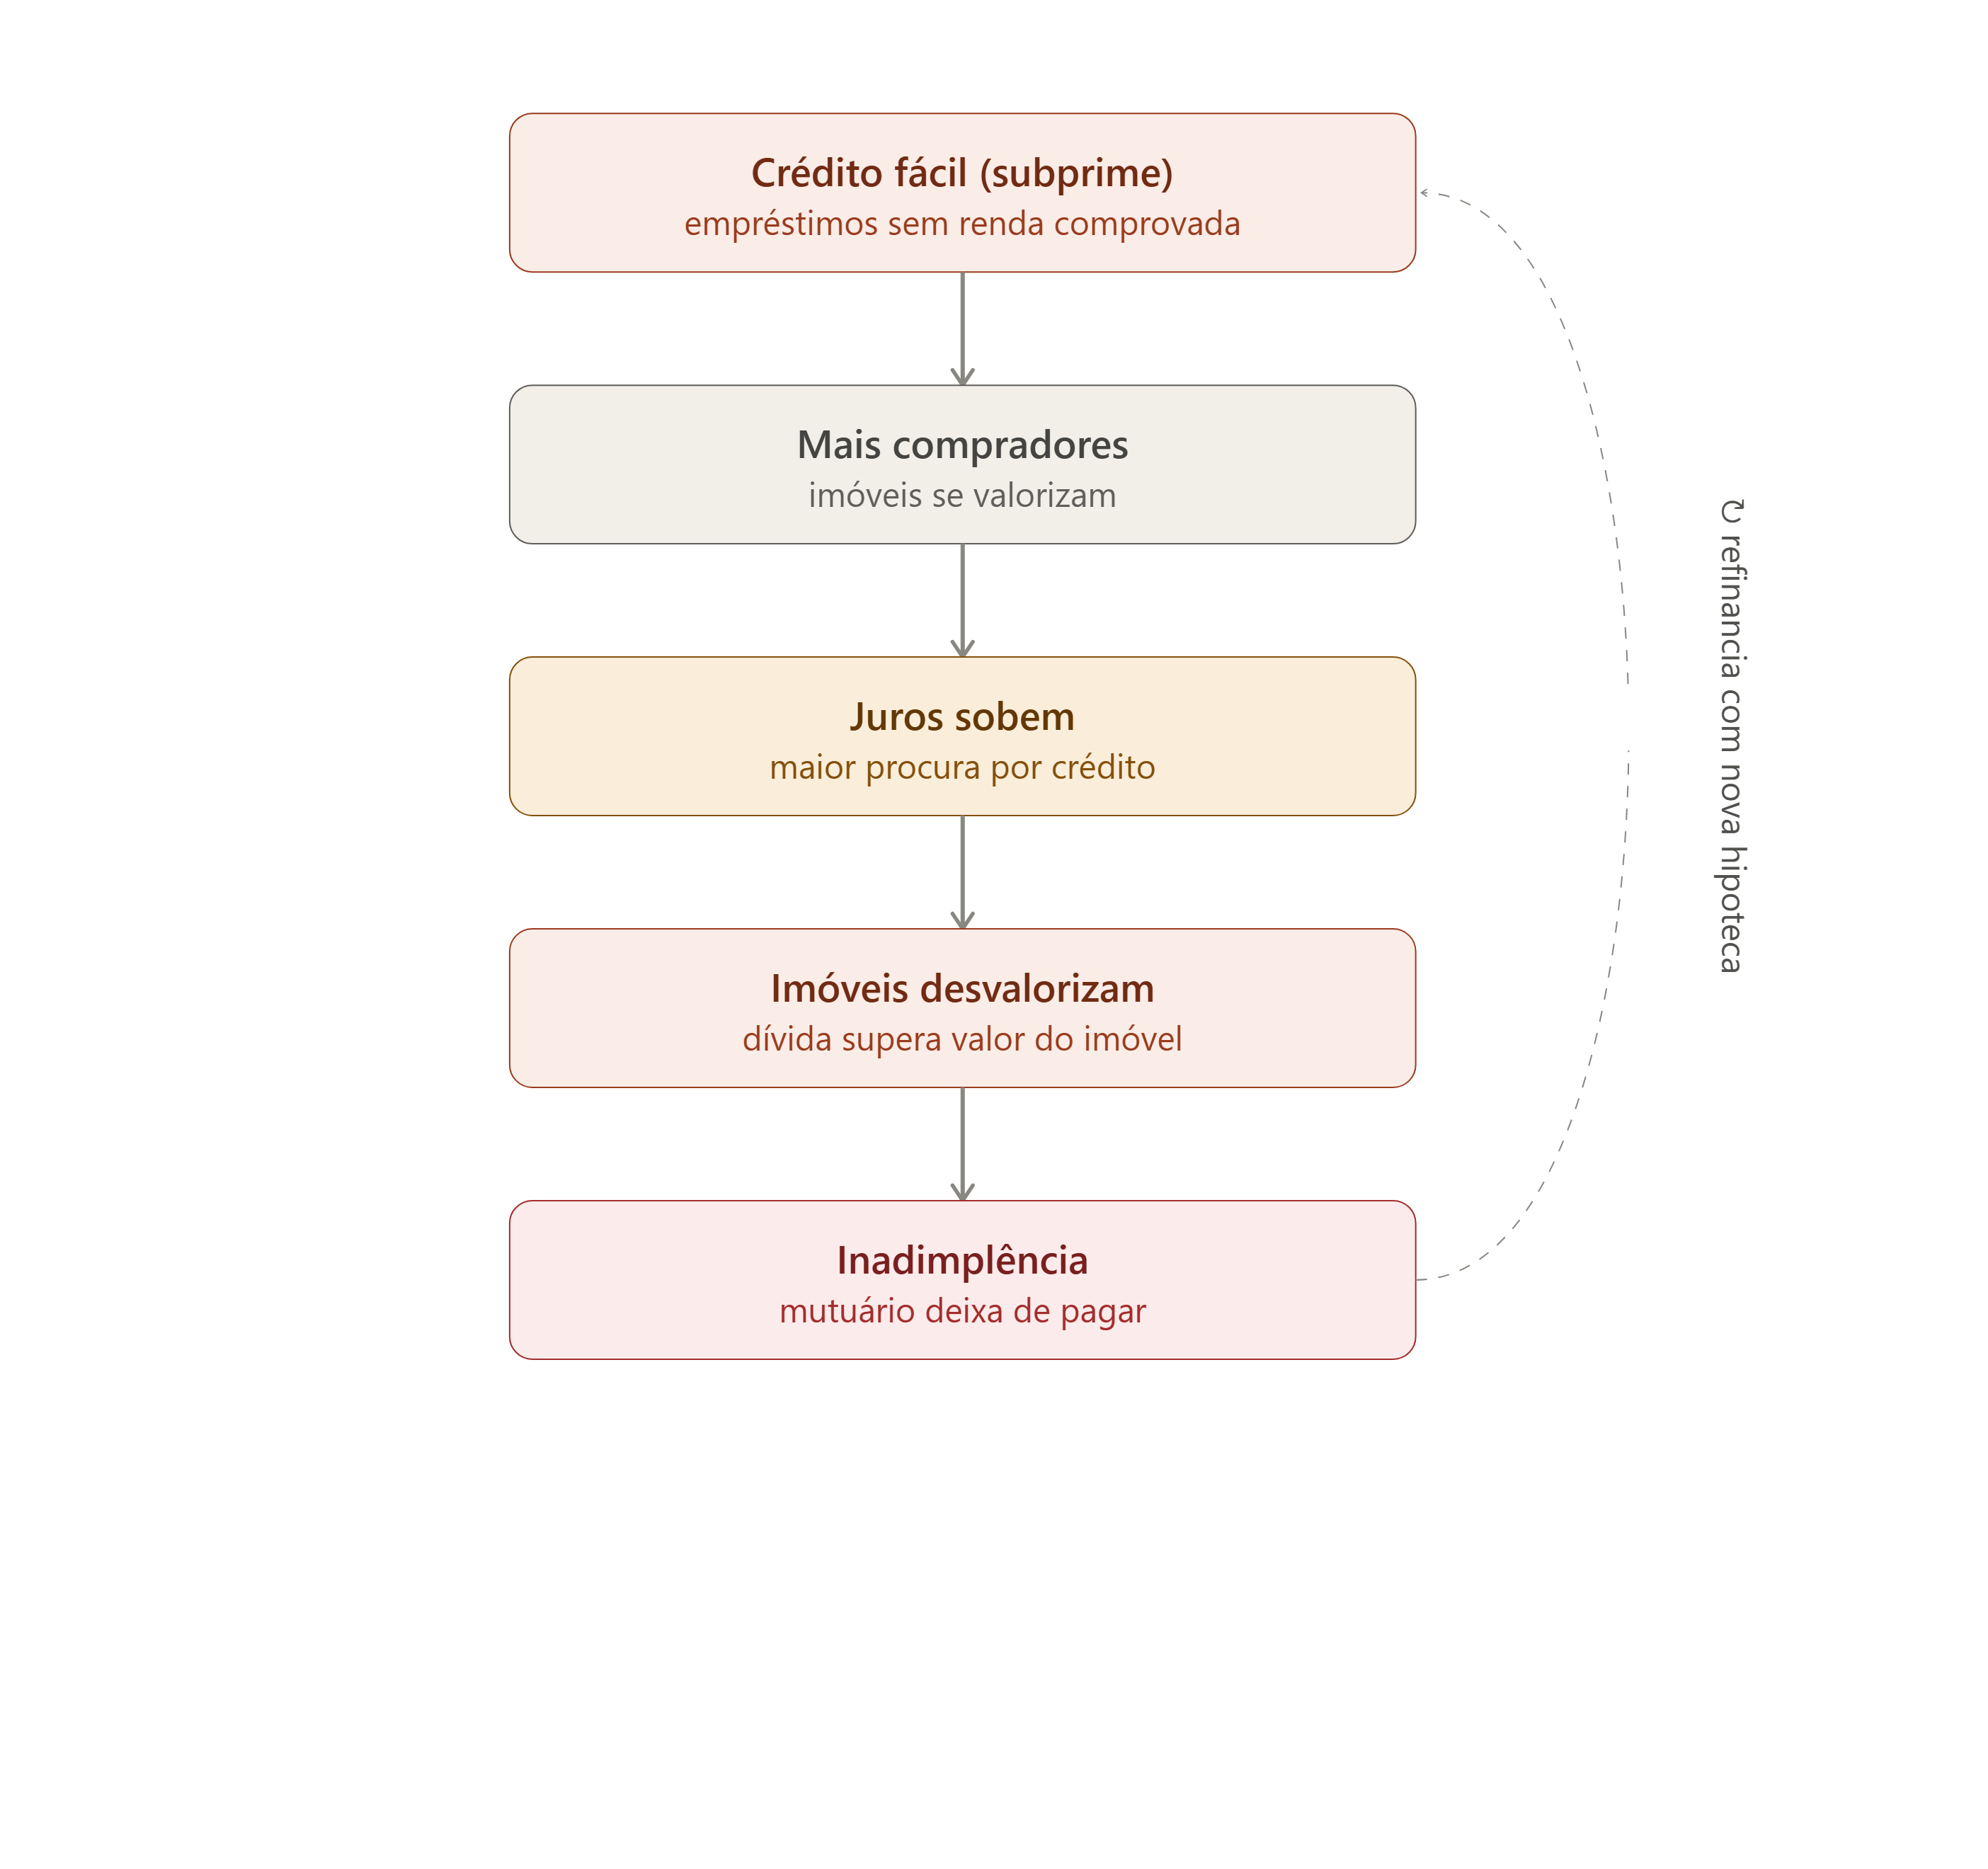
\includegraphics[width=\linewidth]{figuras/ciclo_mercado_imobiliario_2008.png}

\column{0.49\textwidth}
\centering
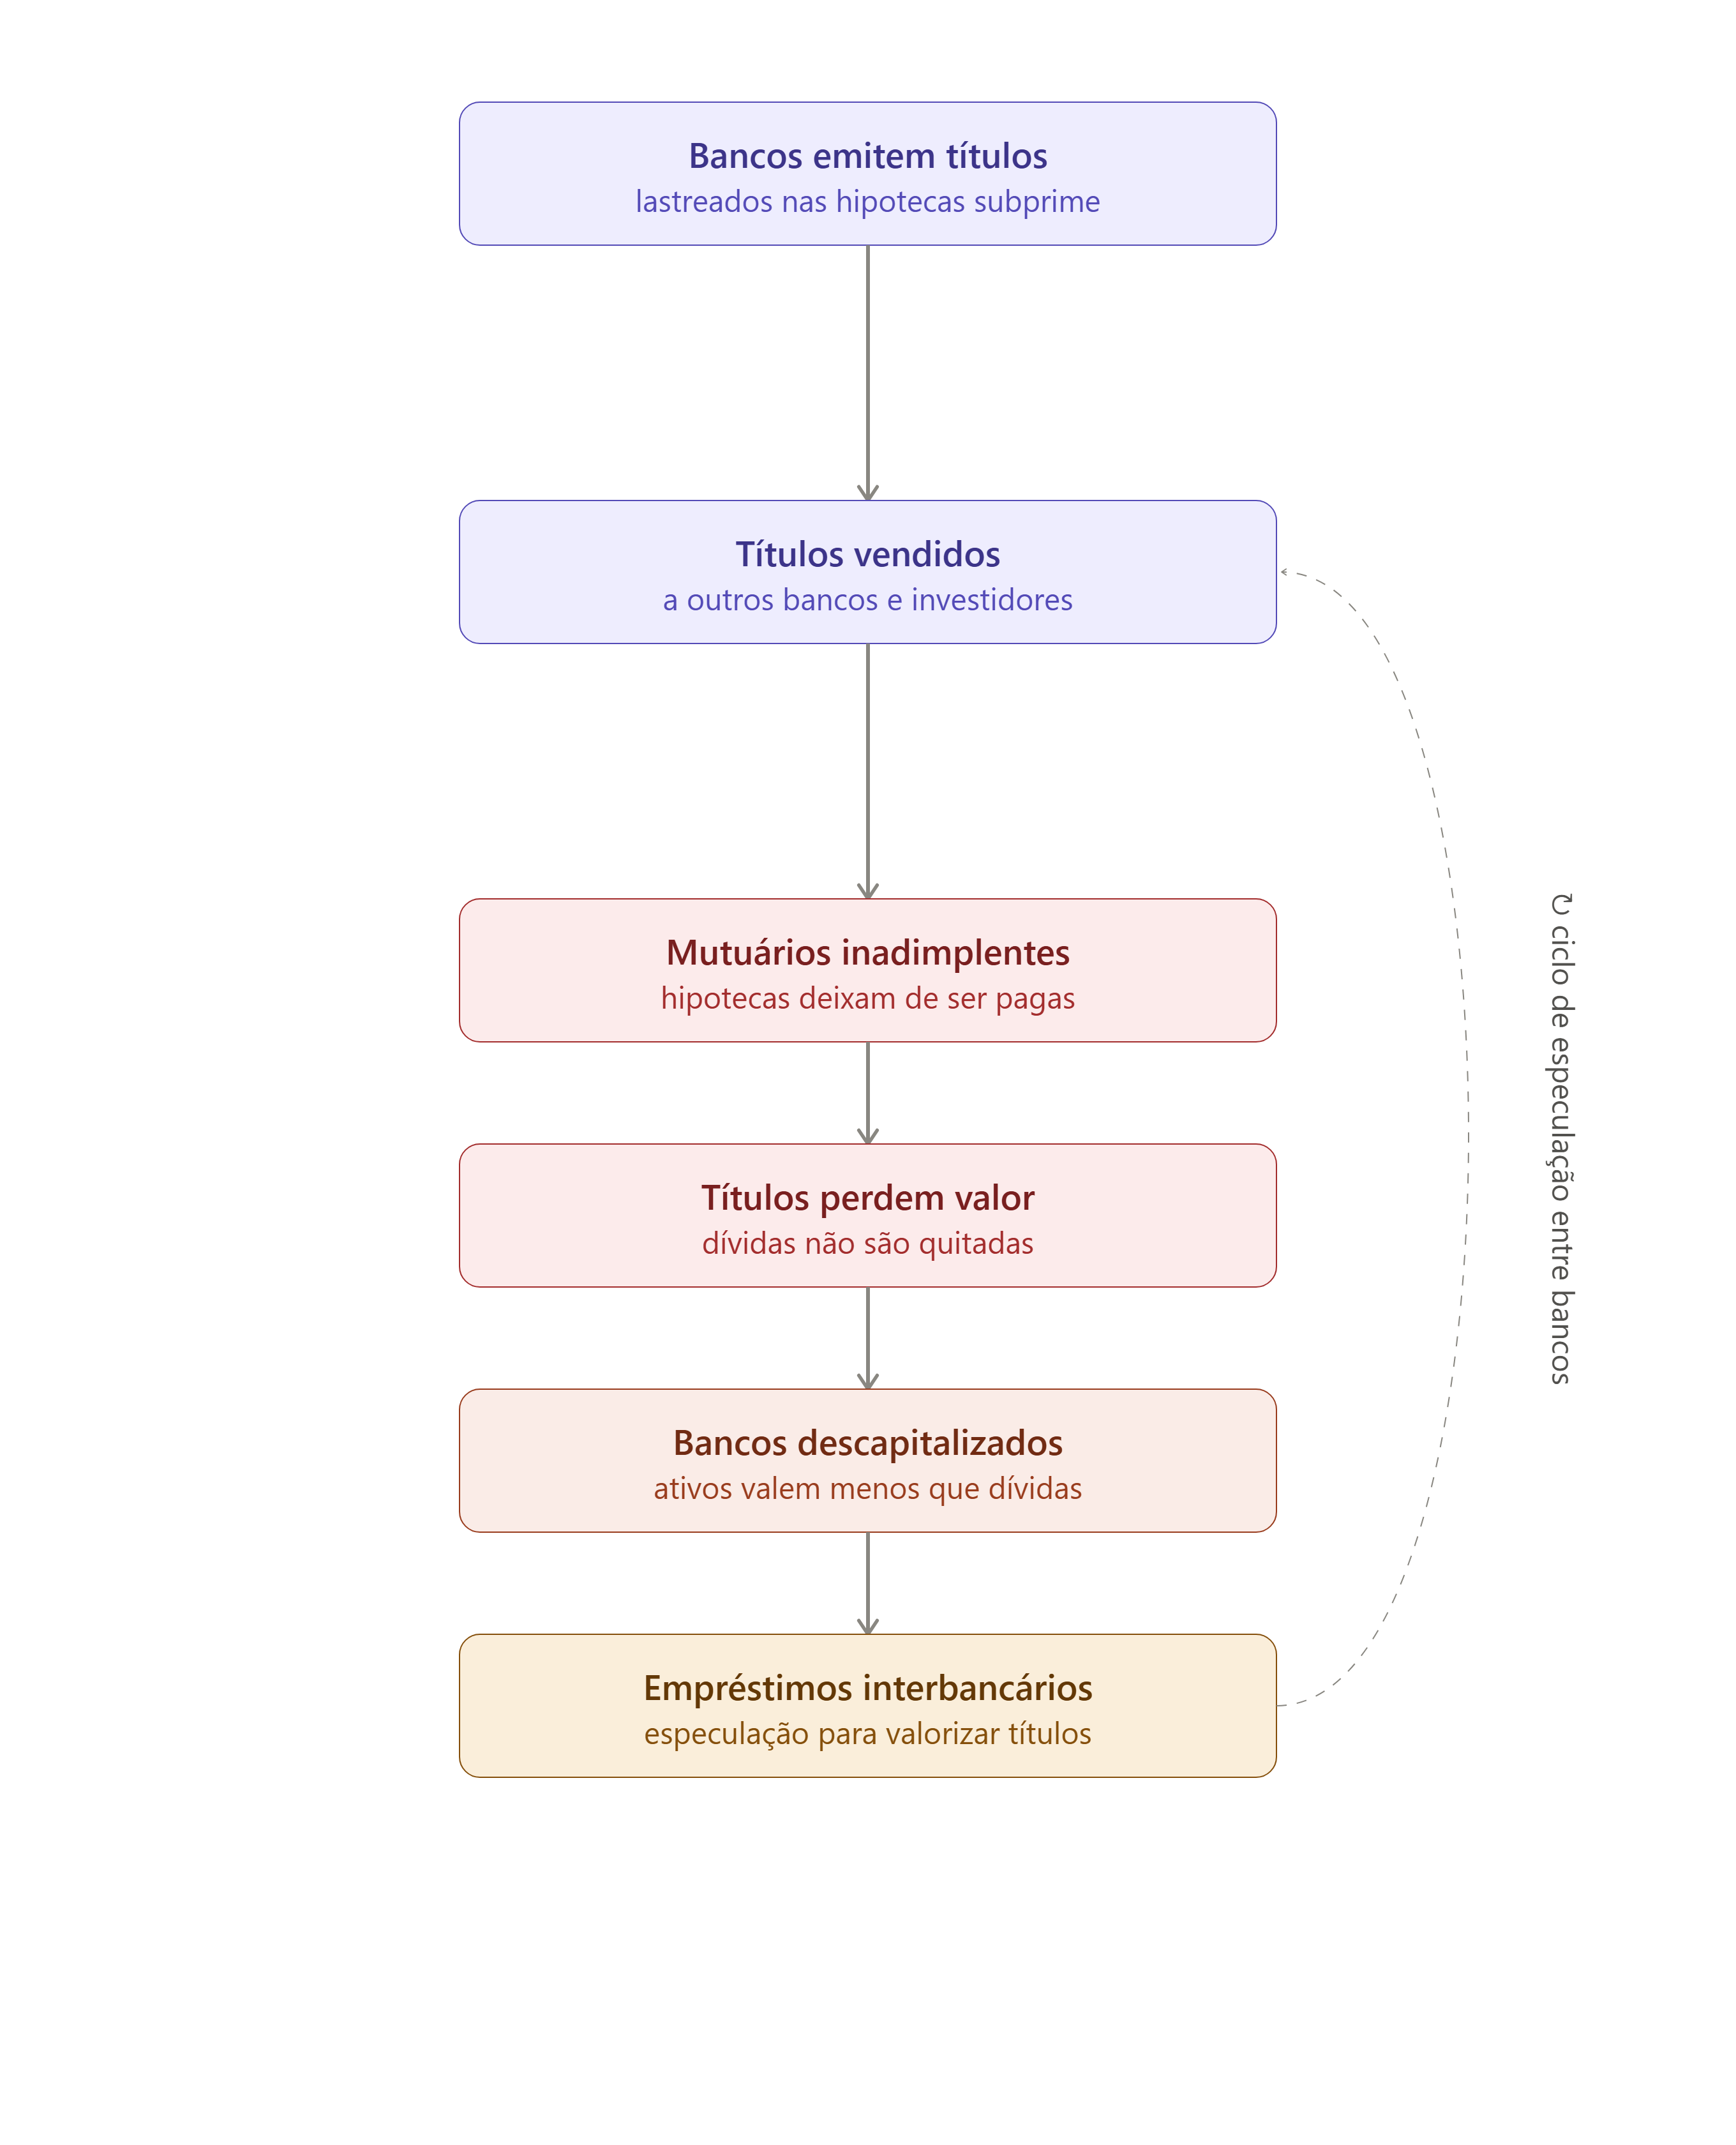
\includegraphics[height=0.78\textheight,keepaspectratio]{figuras/contagio_sistema_financeiro_2008.png}
\end{columns} 
\end{frame}
\begin{frame}{Impactos Internos}

\end{document}



